\section{Introduction}
\label{sec:intro}

Large language models (LLMs) have accelerated advancements in fields ranging from natural language processing \cite{llama2} to scientific modeling \cite{hyenadna}.
However, the largest LLMs have hundreds of billions of parameters that can take over a terabyte of memory to load in half-precision; this size poses significant challenges for the practical deployment of LLMs \cite{llama1,mixtral,falcon}.
For example, small-batch autoregressive decoding, a common form of inference for LLMs, is memory bound \cite{tseng2024quip}.
Even on a modern datacenter GPU with $\approx 3$TB/s memory bandwidth, a large LLM ($> 200$GB) can only be directly run at $<20$ tokens per second and may require multiple devices \cite{tseng2024quip}.
One way to accelerate inference is by compressing LLMs.
This directly reduces the memory footprint of the model and increases the theoretical maximum inference throughput on any given machine. 

One form of compression, weight-only post-training quantization (PTQ), quantizes trained model weights to lower precision datatypes \cite{dettmers2022scaling,tseng2024quip,chee2023quip}.  
The latest \sota weight-only PTQ methods, \qss and AQLM, use vector quantization (VQ) to achieve high-quality 2-bit models \cite{tseng2024quip,aqlm}.
In VQ, a vector $x \in \mathbb{R}^d$ is quantized to one of $2^{kd}$ vectors in $\mathbb{R}^d$ that form a codebook $C \in \mathbb{R}^{2^{kd} \times d}$. 
A higher vector dimension $d$ allows for better codebook shaping and packing density, improving information utilization \cite{6145679}.
However, unstructured VQ requires exponential time and space in both the bitrate and dimension, limiting its practicality.
During quantization, VQ costs $O(2^{kd}d)$ time to perform nearest-neighbor rounding to $C$, and during inference, $C$ must fit in hardware cache for fast lookups.
This exponential scaling limits how high $d$ can be and thus the advantages of VQ over scalar quantization.

To address this limitation, we propose \qt, which uses trellis-coded quantization (TCQ) to enable tractable ultra-high-dimensional ($>100$) quantization and improve quantization quality over prior VQ-based approaches.
In the simplest scalar form of TCQ, a length-$T$ sequence $S$ is \textit{statefully} quantized using a trellis -- a directed graph $G$ with $2^L$ nodes, each with $2^k$ incoming and outgoing edges and a scalar value \cite{46532}.
The reconstructed sequence $\hat S$ corresponds to the node values of a length-$T$ walk on $G$, and quantization finds the walk that minimizes some distortion metric on $S$ and $\hat S$.
Since neighboring entries in $\hat S$ are connected by one of $2^k$ edges, we only need to store \textit{which edge} an entry came from, which takes $k$ bits. 
For additive distortion metrics such as squared error, the optimal $\hat S$ can be found with the Viterbi algorithm, which runs in $O(2^L T)$ time \cite{1450960,46532}.
This means that the cost of quantization is \textit{independent} of the bitrate $k$ and \textit{linear} in the sequence dimension $T$, enabling tractable high dimensional quantization.

However, TCQ is not free. 
During inference, vanilla TCQ requires storing both $G$ and the size $2^{L}\times V$ node value codebook, which can be too large to fit in cache. 
TCQ-quantized sequences also cannot generally be decoded in parallel, as $t$th elment of $\hat S$ could depend on up to the first $tk$ encoded bits.
In \qt, we solve these issues by introducing a series of fast compute-based Gaussian codes designed for the hardware-efficient ``bitshift trellis.''
Specifically, the bitshift trellis supports parallel decoding, does not require storing $G$, and our compute-based codes eliminate needing to store a large node value codebook.
This enables high-quality quantization of Gaussian sources while supporting fast inference, and we adopt incoherence processing with the random Hadamard transform to ensure that LLM weights are approximately i.i.d Gaussian distributed. 
Altogether, \qt
\begin{enumerate}
\item Achieves a \sota combination of weight-only LLM PTQ quality and fast inference through hardware-efficient trellis and codebook design.
\item Introduces multiple novel hardware-efficient ($\le 4$ instructions per weight) compute-based random Gaussian codes for TCQ on i.i.d.\ Gaussian sources.
\end{enumerate}




\begin{figure}
$\vcenter{\hbox{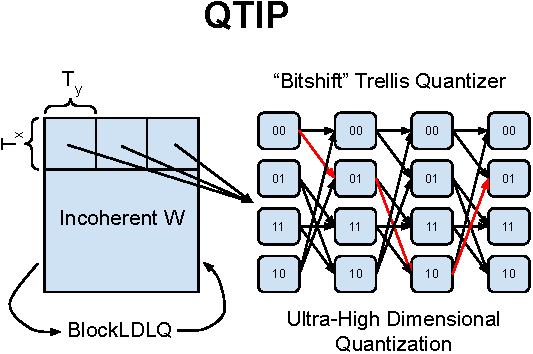
\includegraphics[width=0.52\linewidth]{images/qtip.pdf}}}$
\hspace{0.02\linewidth}
$\vcenter{\hbox{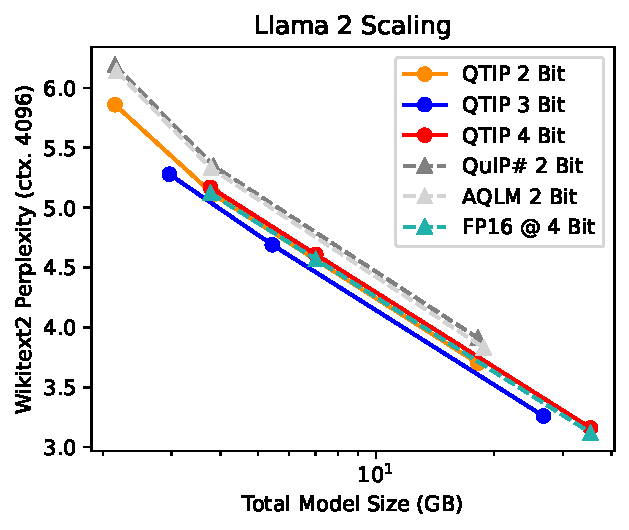
\includegraphics[width=0.46\linewidth]{images/plot.pdf}}}$
\caption{\qts performs ultra-high dimensional ($>100$) quantization by using Trellis Coded Quantization, which has linear cost in dimension. This enables \qts to outperform Vector Quantization-based approaches (\qs, AQLM) that are limited to low dimensions. With QTIP, 2 bit models scale better than theoretically optimal 4 bit models.}
\end{figure}
